% Copy this file to start a new note. Builds with pdflatex (the default recipe).
\documentclass[11pt]{article}
\usepackage{quicknotes}

\title{Data Science 6}
\author{Mark}
\date{}

\begin{document}
\maketitle

% \lecture{number}{date}{topic}
\lecture{1}{Monday, June 30, 2026}{Introduction}

W.E Du Bois graphs post encmapaction. Data can explore, infer, and predict. 
\section{Intro}
\subsection{Exploration}

Abstraction (taking large data and abstacting it to simplfy) and Algorithmic thinking (creating systems to process data). 
Mostly what are we doing in this class. Ex: graphs from berkeley during covid

Bias in depixlation graphs, based on bias traning data (white features) and also hallucinations. 

Look at data6.org and datahub.berkeley.edu for hw and lecs and gradescope. 

\section{What are computer programs}

What is python: bassically a lanauge that is simplefed then by the computer to run. Using jupyter notebooks instead of ides.  We will use datahub.berkeley.edu on a berkeley hosted server that runs jupyer notebooks.

\subsection{Arithmetic}
Expressions are evaluated from left to right
\begin{itemize}
    \item Expressions have values (2) and operators (like + and **)
    \item Expressions evaluate to values
\end{itemize}

Ex: $\text{pow}(2,3) \rightarrow 8$

Syntax rules are like PEMDAS for math, python uses PEMDAS to eval math expressions. Recall the basic operators. 

\begin{figure}[h]
    \centering
    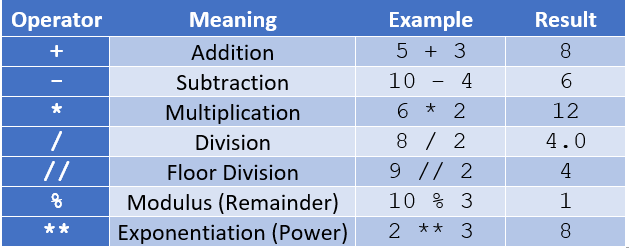
\includegraphics[width=0.7\textwidth]{image.png}
    \caption{Common Python Operators}
    \label{fig:label}
\end{figure}

Note our number system is base 10. So modulating a number by 10 gives the last digit and flooring the number by 10 gives everything but the last digit.
\begin{note}
    \itshape  Shift + enter to run quickly. Also only last evaluated command is outputed.
\end{note}

\lookup[] Edit vs command mode

USE COMMENTS to tell you what the code acutally does. Good practice. 

\subsection{Data Types}
Do diffrent things and have diffrent limts, consider when to use them and the benifits. 
\begin{itemize}
    \item ints
    \item floats
    \item booleans
    \item strings
\end{itemize}

\begin{note}
    \itshape REMEMBER Exps return ints when use only ints unless a float is used 
\end{note}
% Start typing. In math mode the snippets do the work:
% \[
%     \lim_{x \to 0} \frac{\sin x}{x} = 1
% \]

% \begin{definition}
% A function $f$ is continuous at $a$ if $\lim_{x \to a} f(x) = f(a)$.
% \end{definition}

% \begin{theorem}[Pythagoras]
% For a right triangle, $a^2 + b^2 = c^2$.
% \end{theorem}

\section*{Quick quiz --- check your understanding}
\begin{enumerate}
    \item What are the two core skills for working with data that this class emphasises, and what does each mean?
    \item Give two reasons the depixelation / image models produced biased results.
    \item In what order does Python evaluate an expression, and what rule governs the precedence of the math operators?
    \item What does \verb|pow(2, 3)| evaluate to? Which operator gives the same result?
    \item Our numbers are base~10. What does \verb|n % 10| give you? What does \verb|n // 10| (floor) give you?
    \item In a Jupyter notebook: which keystroke runs a cell quickly, and how many of the cell's expressions get displayed as output?
    \item List the four basic data types introduced.
    \item If an expression uses only \texttt{int}s, what type does it return --- and what one thing changes that?
\end{enumerate}

\newpage
\section*{Answers}
\begin{enumerate}
    \item \emph{Abstraction} (simplifying large data down to what matters) and \emph{algorithmic thinking} (building systems/steps to process data).
    \item Biased training data (features skewed toward white faces) and model \emph{hallucination} --- it invents plausible-but-wrong detail.
    \item Left to right, following \textbf{PEMDAS} for operator precedence.
    \item \verb|pow(2, 3)| $= 8$; the equivalent operator is \verb|**| (i.e.\ \verb|2 ** 3|).
    \item \verb|n % 10| gives the \emph{last digit}; \verb|n // 10| gives \emph{everything except the last digit}.
    \item \texttt{Shift + Enter}; only the \emph{last} evaluated expression in the cell is shown.
    \item \texttt{int}, \texttt{float}, \texttt{boolean}, \texttt{string}.
    \item It returns an \texttt{int} --- unless a \texttt{float} appears anywhere in the expression, which makes the result a \texttt{float}.
\end{enumerate}

\end{document}
